% Options for packages loaded elsewhere
\PassOptionsToPackage{unicode}{hyperref}
\PassOptionsToPackage{hyphens}{url}
%
\documentclass[
]{article}
\usepackage{lmodern}
\usepackage{amsmath}
\usepackage{ifxetex,ifluatex}
\ifnum 0\ifxetex 1\fi\ifluatex 1\fi=0 % if pdftex
  \usepackage[T1]{fontenc}
  \usepackage[utf8]{inputenc}
  \usepackage{textcomp} % provide euro and other symbols
  \usepackage{amssymb}
\else % if luatex or xetex
  \usepackage{unicode-math}
  \defaultfontfeatures{Scale=MatchLowercase}
  \defaultfontfeatures[\rmfamily]{Ligatures=TeX,Scale=1}
\fi
% Use upquote if available, for straight quotes in verbatim environments
\IfFileExists{upquote.sty}{\usepackage{upquote}}{}
\IfFileExists{microtype.sty}{% use microtype if available
  \usepackage[]{microtype}
  \UseMicrotypeSet[protrusion]{basicmath} % disable protrusion for tt fonts
}{}
\makeatletter
\@ifundefined{KOMAClassName}{% if non-KOMA class
  \IfFileExists{parskip.sty}{%
    \usepackage{parskip}
  }{% else
    \setlength{\parindent}{0pt}
    \setlength{\parskip}{6pt plus 2pt minus 1pt}}
}{% if KOMA class
  \KOMAoptions{parskip=half}}
\makeatother
\usepackage{xcolor}
\IfFileExists{xurl.sty}{\usepackage{xurl}}{} % add URL line breaks if available
\IfFileExists{bookmark.sty}{\usepackage{bookmark}}{\usepackage{hyperref}}
\hypersetup{
  pdftitle={Final Project},
  pdfauthor={London Wagner, Erik Lovece, Carmen Canedo},
  hidelinks,
  pdfcreator={LaTeX via pandoc}}
\urlstyle{same} % disable monospaced font for URLs
\usepackage[margin=1in]{geometry}
\usepackage{color}
\usepackage{fancyvrb}
\newcommand{\VerbBar}{|}
\newcommand{\VERB}{\Verb[commandchars=\\\{\}]}
\DefineVerbatimEnvironment{Highlighting}{Verbatim}{commandchars=\\\{\}}
% Add ',fontsize=\small' for more characters per line
\usepackage{framed}
\definecolor{shadecolor}{RGB}{248,248,248}
\newenvironment{Shaded}{\begin{snugshade}}{\end{snugshade}}
\newcommand{\AlertTok}[1]{\textcolor[rgb]{0.94,0.16,0.16}{#1}}
\newcommand{\AnnotationTok}[1]{\textcolor[rgb]{0.56,0.35,0.01}{\textbf{\textit{#1}}}}
\newcommand{\AttributeTok}[1]{\textcolor[rgb]{0.77,0.63,0.00}{#1}}
\newcommand{\BaseNTok}[1]{\textcolor[rgb]{0.00,0.00,0.81}{#1}}
\newcommand{\BuiltInTok}[1]{#1}
\newcommand{\CharTok}[1]{\textcolor[rgb]{0.31,0.60,0.02}{#1}}
\newcommand{\CommentTok}[1]{\textcolor[rgb]{0.56,0.35,0.01}{\textit{#1}}}
\newcommand{\CommentVarTok}[1]{\textcolor[rgb]{0.56,0.35,0.01}{\textbf{\textit{#1}}}}
\newcommand{\ConstantTok}[1]{\textcolor[rgb]{0.00,0.00,0.00}{#1}}
\newcommand{\ControlFlowTok}[1]{\textcolor[rgb]{0.13,0.29,0.53}{\textbf{#1}}}
\newcommand{\DataTypeTok}[1]{\textcolor[rgb]{0.13,0.29,0.53}{#1}}
\newcommand{\DecValTok}[1]{\textcolor[rgb]{0.00,0.00,0.81}{#1}}
\newcommand{\DocumentationTok}[1]{\textcolor[rgb]{0.56,0.35,0.01}{\textbf{\textit{#1}}}}
\newcommand{\ErrorTok}[1]{\textcolor[rgb]{0.64,0.00,0.00}{\textbf{#1}}}
\newcommand{\ExtensionTok}[1]{#1}
\newcommand{\FloatTok}[1]{\textcolor[rgb]{0.00,0.00,0.81}{#1}}
\newcommand{\FunctionTok}[1]{\textcolor[rgb]{0.00,0.00,0.00}{#1}}
\newcommand{\ImportTok}[1]{#1}
\newcommand{\InformationTok}[1]{\textcolor[rgb]{0.56,0.35,0.01}{\textbf{\textit{#1}}}}
\newcommand{\KeywordTok}[1]{\textcolor[rgb]{0.13,0.29,0.53}{\textbf{#1}}}
\newcommand{\NormalTok}[1]{#1}
\newcommand{\OperatorTok}[1]{\textcolor[rgb]{0.81,0.36,0.00}{\textbf{#1}}}
\newcommand{\OtherTok}[1]{\textcolor[rgb]{0.56,0.35,0.01}{#1}}
\newcommand{\PreprocessorTok}[1]{\textcolor[rgb]{0.56,0.35,0.01}{\textit{#1}}}
\newcommand{\RegionMarkerTok}[1]{#1}
\newcommand{\SpecialCharTok}[1]{\textcolor[rgb]{0.00,0.00,0.00}{#1}}
\newcommand{\SpecialStringTok}[1]{\textcolor[rgb]{0.31,0.60,0.02}{#1}}
\newcommand{\StringTok}[1]{\textcolor[rgb]{0.31,0.60,0.02}{#1}}
\newcommand{\VariableTok}[1]{\textcolor[rgb]{0.00,0.00,0.00}{#1}}
\newcommand{\VerbatimStringTok}[1]{\textcolor[rgb]{0.31,0.60,0.02}{#1}}
\newcommand{\WarningTok}[1]{\textcolor[rgb]{0.56,0.35,0.01}{\textbf{\textit{#1}}}}
\usepackage{graphicx}
\makeatletter
\def\maxwidth{\ifdim\Gin@nat@width>\linewidth\linewidth\else\Gin@nat@width\fi}
\def\maxheight{\ifdim\Gin@nat@height>\textheight\textheight\else\Gin@nat@height\fi}
\makeatother
% Scale images if necessary, so that they will not overflow the page
% margins by default, and it is still possible to overwrite the defaults
% using explicit options in \includegraphics[width, height, ...]{}
\setkeys{Gin}{width=\maxwidth,height=\maxheight,keepaspectratio}
% Set default figure placement to htbp
\makeatletter
\def\fps@figure{htbp}
\makeatother
\setlength{\emergencystretch}{3em} % prevent overfull lines
\providecommand{\tightlist}{%
  \setlength{\itemsep}{0pt}\setlength{\parskip}{0pt}}
\setcounter{secnumdepth}{5}
\ifluatex
  \usepackage{selnolig}  % disable illegal ligatures
\fi

\title{Final Project}
\author{London Wagner, Erik Lovece, Carmen Canedo}
\date{2021-04-25}

\begin{document}
\maketitle

\hypertarget{introduction}{%
\section{Introduction}\label{introduction}}

Our final project analyzes the student performance dataset from the UCI
Machine Learning Repository, originally gathered by Paulo Cortez from
the University of Minho. This dataset measures the final student grade
in a Portuguese class based on a variety of predictors. These predictors
cover numerous aspects of not only students' academic lives, but also
family life predictors such as parental employment, and personal
predictors like whether or not they have home internet access and
whether or not they are in a romantic relationship.

We seek to answer the question of what predictors have the greatest
influence in how a student does in class. Conventional wisdom seems to
dictate that high-achieving students have come from particularly
favorable academic, filial, and personal environments, and previous
studies have confirmed this. Our model, if properly constructed along
the best machine learning practices, should corroborate this, although
unexpected conclusions may also lie in store.

Our workflow for finding a sufficient model from which we will draw our
conclusions is as follows:

\begin{enumerate}
\def\labelenumi{\arabic{enumi})}
\tightlist
\item
  Run a linear regression model with final grade as the response and all
  other variables as predictors
\item
  Use best subset, forward step, and backwards step to select variables
  for a reduced model
\item
  Use ridge, lasso, principal component regression, and partial least
  squares regression to conduct further dimension reduction
\item
  Use cross validation methods to determine which model predicts the
  final grade with the greatest accuracy
\item
  Make more definitive determinations based on the chosen model.
\end{enumerate}

\hypertarget{loading-data}{%
\section{Loading Data}\label{loading-data}}

\begin{Shaded}
\begin{Highlighting}[]
\NormalTok{student\_por }\OtherTok{\textless{}{-}} \FunctionTok{read\_csv2}\NormalTok{(}\StringTok{"data/student{-}por.csv"}\NormalTok{)}

\NormalTok{student\_por}
\end{Highlighting}
\end{Shaded}

\begin{verbatim}
## # A tibble: 649 x 33
##    school sex     age address famsize Pstatus  Medu  Fedu Mjob    Fjob   reason 
##    <chr>  <chr> <dbl> <chr>   <chr>   <chr>   <dbl> <dbl> <chr>   <chr>  <chr>  
##  1 GP     F        18 U       GT3     A           4     4 at_home teach~ course 
##  2 GP     F        17 U       GT3     T           1     1 at_home other  course 
##  3 GP     F        15 U       LE3     T           1     1 at_home other  other  
##  4 GP     F        15 U       GT3     T           4     2 health  servi~ home   
##  5 GP     F        16 U       GT3     T           3     3 other   other  home   
##  6 GP     M        16 U       LE3     T           4     3 servic~ other  reputa~
##  7 GP     M        16 U       LE3     T           2     2 other   other  home   
##  8 GP     F        17 U       GT3     A           4     4 other   teach~ home   
##  9 GP     M        15 U       LE3     A           3     2 servic~ other  home   
## 10 GP     M        15 U       GT3     T           3     4 other   other  home   
## # ... with 639 more rows, and 22 more variables: guardian <chr>,
## #   traveltime <dbl>, studytime <dbl>, failures <dbl>, schoolsup <chr>,
## #   famsup <chr>, paid <chr>, activities <chr>, nursery <chr>, higher <chr>,
## #   internet <chr>, romantic <chr>, famrel <dbl>, freetime <dbl>, goout <dbl>,
## #   Dalc <dbl>, Walc <dbl>, health <dbl>, absences <dbl>, G1 <dbl>, G2 <dbl>,
## #   G3 <dbl>
\end{verbatim}

The student attributes and grades forming the predictors and response,
quoted verbatim from a text file provided with the dataset, are as
follows:

1 school - student's school (binary: ``GP'' - Gabriel Pereira or ``MS''
- Mousinho da Silveira)

2 sex - student's sex (binary: ``F'' - female or ``M'' - male)

3 age - student's age (numeric: from 15 to 22)

4 address - student's home address type (binary: ``U'' - urban or ``R''
- rural)

5 famsize - family size (binary: ``LE3'' - less or equal to 3 or ``GT3''
- greater than 3)

6 Pstatus - parent's cohabitation status (binary: ``T'' - living
together or ``A'' - apart)

7 Medu - mother's education (numeric: 0 - none, 1 - primary education
(4th grade), 2 -- 5th to 9th grade, 3 -- secondary education or 4 --
higher education)

8 Fedu - father's education (numeric: 0 - none, 1 - primary education
(4th grade), 2 -- 5th to 9th grade, 3 -- secondary education or 4 --
higher education)

9 Mjob - mother's job (nominal: ``teacher'', ``health'' care related,
civil ``services'' (e.g.~administrative or police), ``at\_home'' or
``other'')

10 Fjob - father's job (nominal: ``teacher'', ``health'' care related,
civil ``services'' (e.g.~administrative or police), ``at\_home'' or
``other'')

11 reason - reason to choose this school (nominal: close to ``home'',
school ``reputation'', ``course'' preference or ``other'')

12 guardian - student's guardian (nominal: ``mother'', ``father'' or
``other'')

13 traveltime - home to school travel time (numeric: 1 - \textless15
min., 2 - 15 to 30 min., 3 - 30 min. to 1 hour, or 4 - \textgreater1
hour)

14 studytime - weekly study time (numeric: 1 - \textless2 hours, 2 - 2
to 5 hours, 3 - 5 to 10 hours, or 4 - \textgreater10 hours)

15 failures - number of past class failures (numeric: n if
1\textless=n\textless3, else 4)

16 schoolsup - extra educational support (binary: yes or no)

17 famsup - family educational support (binary: yes or no)

18 paid - extra paid classes within the course subject (Math or
Portuguese) (binary: yes or no)

19 activities - extra-curricular activities (binary: yes or no)

20 nursery - attended nursery school (binary: yes or no)

21 higher - wants to take higher education (binary: yes or no)

22 internet - Internet access at home (binary: yes or no)

23 romantic - with a romantic relationship (binary: yes or no)

24 famrel - quality of family relationships (numeric: from 1 - very bad
to 5 - excellent)

25 freetime - free time after school (numeric: from 1 - very low to 5 -
very high)

26 goout - going out with friends (numeric: from 1 - very low to 5 -
very high)

27 Dalc - workday alcohol consumption (numeric: from 1 - very low to 5 -
very high)

28 Walc - weekend alcohol consumption (numeric: from 1 - very low to 5 -
very high)

29 health - current health status (numeric: from 1 - very bad to 5 -
very good)

30 absences - number of school absences (numeric: from 0 to 93)

31 G1 - first period grade (numeric: from 0 to 20)

31 G2 - second period grade (numeric: from 0 to 20)

32 G3 - final grade (numeric: from 0 to 20, output target)

For all of our models, \texttt{G3} is our response and every other
variable serves as a predictor (pending elimination).

\hypertarget{data-cleaning}{%
\section{Data Cleaning}\label{data-cleaning}}

When creating our models, some variables need be converting to factors
in order to be properly interpreted by the \texttt{lm} function. We have
converted the necessary variables, so now many of them (with special
emphasis on binary variables) are now of type factor.

\begin{Shaded}
\begin{Highlighting}[]
\NormalTok{student\_por}
\end{Highlighting}
\end{Shaded}

\begin{verbatim}
## # A tibble: 649 x 33
##    school sex     age address famsize Pstatus  Medu  Fedu Mjob    Fjob   reason 
##    <fct>  <fct> <dbl> <fct>   <fct>   <fct>   <dbl> <dbl> <chr>   <chr>  <fct>  
##  1 GP     F        18 U       GT3     A           4     4 at_home teach~ course 
##  2 GP     F        17 U       GT3     T           1     1 at_home other  course 
##  3 GP     F        15 U       LE3     T           1     1 at_home other  other  
##  4 GP     F        15 U       GT3     T           4     2 health  servi~ home   
##  5 GP     F        16 U       GT3     T           3     3 other   other  home   
##  6 GP     M        16 U       LE3     T           4     3 servic~ other  reputa~
##  7 GP     M        16 U       LE3     T           2     2 other   other  home   
##  8 GP     F        17 U       GT3     A           4     4 other   teach~ home   
##  9 GP     M        15 U       LE3     A           3     2 servic~ other  home   
## 10 GP     M        15 U       GT3     T           3     4 other   other  home   
## # ... with 639 more rows, and 22 more variables: guardian <chr>,
## #   traveltime <dbl>, studytime <dbl>, failures <dbl>, schoolsup <fct>,
## #   famsup <fct>, paid <fct>, activities <fct>, nursery <fct>, higher <fct>,
## #   internet <fct>, romantic <fct>, famrel <dbl>, freetime <dbl>, goout <dbl>,
## #   Dalc <dbl>, Walc <dbl>, health <dbl>, absences <dbl>, G1 <dbl>, G2 <dbl>,
## #   G3 <dbl>
\end{verbatim}

\hypertarget{exploratory-data-analysis-checking-assumptions}{%
\section{Exploratory Data Analysis \& Checking
Assumptions}\label{exploratory-data-analysis-checking-assumptions}}

Before we begin our analysis, we wish to explore the distribution of the
data and confirm it follows the typical assumptions of linear
regression. Although we recognize that these assumptions are not as
necessary in machine learning, they can be helpful when determining what
kind of model we should use to predict our response variable, G3.

\begin{Shaded}
\begin{Highlighting}[]
\FunctionTok{summary}\NormalTok{(student\_por)}
\end{Highlighting}
\end{Shaded}

\begin{verbatim}
##  school   sex          age        address famsize   Pstatus      Medu      
##  GP:423   F:383   Min.   :15.00   R:197   GT3:457   A: 80   Min.   :0.000  
##  MS:226   M:266   1st Qu.:16.00   U:452   LE3:192   T:569   1st Qu.:2.000  
##                   Median :17.00                             Median :2.000  
##                   Mean   :16.74                             Mean   :2.515  
##                   3rd Qu.:18.00                             3rd Qu.:4.000  
##                   Max.   :22.00                             Max.   :4.000  
##       Fedu           Mjob               Fjob                  reason   
##  Min.   :0.000   Length:649         Length:649         course    :285  
##  1st Qu.:1.000   Class :character   Class :character   home      :149  
##  Median :2.000   Mode  :character   Mode  :character   other     : 72  
##  Mean   :2.307                                         reputation:143  
##  3rd Qu.:3.000                                                         
##  Max.   :4.000                                                         
##    guardian           traveltime      studytime        failures      schoolsup
##  Length:649         Min.   :1.000   Min.   :1.000   Min.   :0.0000   no :581  
##  Class :character   1st Qu.:1.000   1st Qu.:1.000   1st Qu.:0.0000   yes: 68  
##  Mode  :character   Median :1.000   Median :2.000   Median :0.0000            
##                     Mean   :1.569   Mean   :1.931   Mean   :0.2219            
##                     3rd Qu.:2.000   3rd Qu.:2.000   3rd Qu.:0.0000            
##                     Max.   :4.000   Max.   :4.000   Max.   :3.0000            
##  famsup     paid     activities nursery   higher    internet  romantic 
##  no :251   no :610   no :334    no :128   no : 69   no :151   no :410  
##  yes:398   yes: 39   yes:315    yes:521   yes:580   yes:498   yes:239  
##                                                                        
##                                                                        
##                                                                        
##                                                                        
##      famrel         freetime        goout            Dalc            Walc     
##  Min.   :1.000   Min.   :1.00   Min.   :1.000   Min.   :1.000   Min.   :1.00  
##  1st Qu.:4.000   1st Qu.:3.00   1st Qu.:2.000   1st Qu.:1.000   1st Qu.:1.00  
##  Median :4.000   Median :3.00   Median :3.000   Median :1.000   Median :2.00  
##  Mean   :3.931   Mean   :3.18   Mean   :3.185   Mean   :1.502   Mean   :2.28  
##  3rd Qu.:5.000   3rd Qu.:4.00   3rd Qu.:4.000   3rd Qu.:2.000   3rd Qu.:3.00  
##  Max.   :5.000   Max.   :5.00   Max.   :5.000   Max.   :5.000   Max.   :5.00  
##      health         absences            G1             G2       
##  Min.   :1.000   Min.   : 0.000   Min.   : 0.0   Min.   : 0.00  
##  1st Qu.:2.000   1st Qu.: 0.000   1st Qu.:10.0   1st Qu.:10.00  
##  Median :4.000   Median : 2.000   Median :11.0   Median :11.00  
##  Mean   :3.536   Mean   : 3.659   Mean   :11.4   Mean   :11.57  
##  3rd Qu.:5.000   3rd Qu.: 6.000   3rd Qu.:13.0   3rd Qu.:13.00  
##  Max.   :5.000   Max.   :32.000   Max.   :19.0   Max.   :19.00  
##        G3       
##  Min.   : 0.00  
##  1st Qu.:10.00  
##  Median :12.00  
##  Mean   :11.91  
##  3rd Qu.:14.00  
##  Max.   :19.00
\end{verbatim}

Most noteworthy is how G1, G2, and G3's \(1^{st}\) quartile of 10 is
quite close to the median and mean on the 0-20 scale, yet the minimum in
all three is zero. There is a significant gap between the lower and
minimum behavior, and these lowest-end students may influence our
subsequent analyses in some way.

\begin{Shaded}
\begin{Highlighting}[]
\NormalTok{student\_por }\SpecialCharTok{\%\textgreater{}\%} 
  \FunctionTok{ggplot}\NormalTok{(}\FunctionTok{aes}\NormalTok{(}\AttributeTok{x =}\NormalTok{ G3)) }\SpecialCharTok{+}
  \FunctionTok{geom\_histogram}\NormalTok{()}
\end{Highlighting}
\end{Shaded}

\begin{verbatim}
## `stat_bin()` using `bins = 30`. Pick better value with `binwidth`.
\end{verbatim}

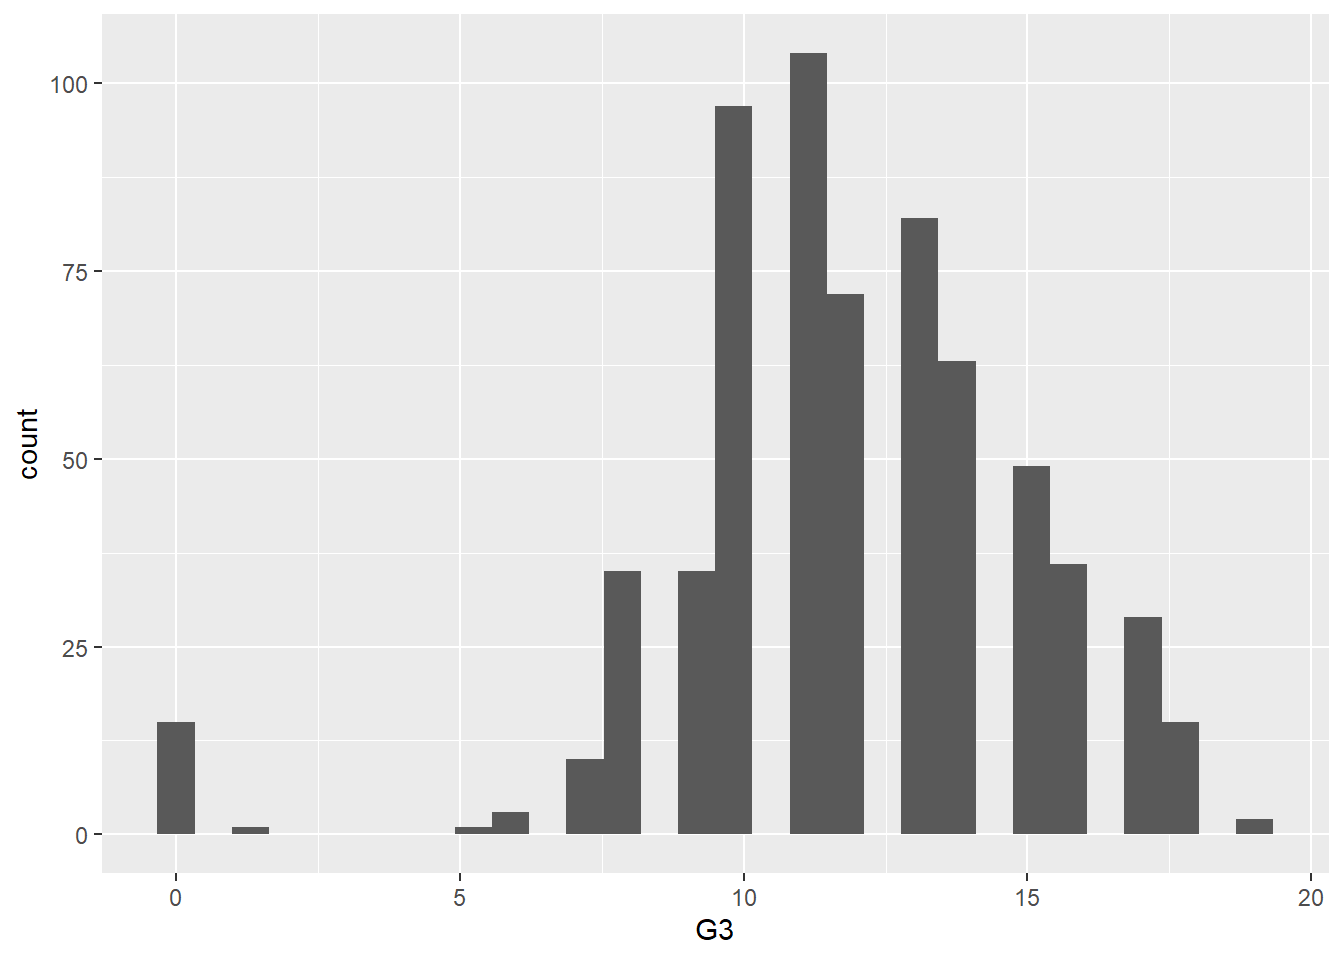
\includegraphics{report_files/figure-latex/unnamed-chunk-6-1.pdf}

\begin{Shaded}
\begin{Highlighting}[]
\NormalTok{lowest }\OtherTok{\textless{}{-}} \FunctionTok{filter}\NormalTok{(student\_por, G3 }\SpecialCharTok{==} \DecValTok{0}\NormalTok{)}
\NormalTok{num\_lowest }\OtherTok{\textless{}{-}} \FunctionTok{nrow}\NormalTok{(lowest)}
\NormalTok{num\_lowest }\SpecialCharTok{/} \FunctionTok{nrow}\NormalTok{(student\_por)}
\end{Highlighting}
\end{Shaded}

\begin{verbatim}
## [1] 0.02311248
\end{verbatim}

\begin{Shaded}
\begin{Highlighting}[]
\NormalTok{lowest}
\end{Highlighting}
\end{Shaded}

\begin{verbatim}
## # A tibble: 15 x 33
##    school sex     age address famsize Pstatus  Medu  Fedu Mjob    Fjob   reason 
##    <fct>  <fct> <dbl> <fct>   <fct>   <fct>   <dbl> <dbl> <chr>   <chr>  <fct>  
##  1 GP     M        18 U       LE3     T           1     1 other   other  course 
##  2 MS     M        16 U       GT3     T           1     1 at_home servi~ home   
##  3 MS     M        16 R       GT3     T           2     1 other   servi~ reputa~
##  4 MS     M        17 U       GT3     T           2     2 other   other  course 
##  5 MS     M        18 R       GT3     T           3     2 servic~ other  course 
##  6 MS     F        18 R       GT3     T           2     2 other   other  other  
##  7 MS     F        17 U       GT3     T           4     2 teacher servi~ home   
##  8 MS     F        18 R       GT3     T           2     2 at_home other  course 
##  9 MS     F        18 R       LE3     A           4     2 teacher other  reputa~
## 10 MS     F        19 U       GT3     T           1     1 at_home servi~ other  
## 11 MS     F        19 R       GT3     A           1     1 at_home at_ho~ course 
## 12 MS     F        18 R       GT3     T           4     4 other   teach~ other  
## 13 MS     M        18 R       GT3     T           2     1 other   other  other  
## 14 MS     M        19 R       GT3     T           1     1 other   servi~ other  
## 15 MS     M        18 R       GT3     T           4     2 other   other  home   
## # ... with 22 more variables: guardian <chr>, traveltime <dbl>,
## #   studytime <dbl>, failures <dbl>, schoolsup <fct>, famsup <fct>, paid <fct>,
## #   activities <fct>, nursery <fct>, higher <fct>, internet <fct>,
## #   romantic <fct>, famrel <dbl>, freetime <dbl>, goout <dbl>, Dalc <dbl>,
## #   Walc <dbl>, health <dbl>, absences <dbl>, G1 <dbl>, G2 <dbl>, G3 <dbl>
\end{verbatim}

As expected, the lowest-performing students left-skew the distribution
of the final scores. However, it is not a couple isolated cases, but
2.3\% of the student population in this class. Although there are some
commonalities among these students (most of them attended nursery school
but did not pay for extra educational support in this subject field, and
they all had zero absences), we will later find that most of these
factors in common are unimportant in our final models. For now, we run
the model taking every student into account.

\hypertarget{running-lm}{%
\subsection{\texorpdfstring{Running
\texttt{lm}}{Running lm}}\label{running-lm}}

\begin{Shaded}
\begin{Highlighting}[]
\NormalTok{por\_reg }\OtherTok{\textless{}{-}} \FunctionTok{lm}\NormalTok{(G3 }\SpecialCharTok{\textasciitilde{}}\NormalTok{ ., }\AttributeTok{data =}\NormalTok{ student\_por)}
\FunctionTok{summary}\NormalTok{(por\_reg)}
\end{Highlighting}
\end{Shaded}

\begin{verbatim}
## 
## Call:
## lm(formula = G3 ~ ., data = student_por)
## 
## Residuals:
##     Min      1Q  Median      3Q     Max 
## -8.7618 -0.5148  0.0038  0.6047  5.4973 
## 
## Coefficients:
##                  Estimate Std. Error t value Pr(>|t|)    
## (Intercept)       0.63823    0.96361   0.662 0.508011    
## schoolMS         -0.19797    0.12783  -1.549 0.121992    
## sexM             -0.12258    0.11778  -1.041 0.298423    
## age               0.02869    0.04835   0.593 0.553208    
## addressU          0.11446    0.12277   0.932 0.351565    
## famsizeLE3        0.01560    0.11505   0.136 0.892197    
## PstatusT         -0.09746    0.16256  -0.600 0.549055    
## Medu             -0.09170    0.07097  -1.292 0.196799    
## Fedu              0.04962    0.06461   0.768 0.442773    
## Mjobhealth        0.26583    0.25225   1.054 0.292379    
## Mjobother        -0.09351    0.14208  -0.658 0.510720    
## Mjobservices      0.17255    0.17510   0.985 0.324808    
## Mjobteacher       0.22115    0.23558   0.939 0.348232    
## Fjobhealth       -0.44420    0.35256  -1.260 0.208189    
## Fjobother        -0.33805    0.21391  -1.580 0.114544    
## Fjobservices     -0.47121    0.22477  -2.096 0.036457 *  
## Fjobteacher      -0.54368    0.31611  -1.720 0.085958 .  
## reasonhome       -0.07885    0.13366  -0.590 0.555479    
## reasonother      -0.36174    0.17236  -2.099 0.036251 *  
## reasonreputation -0.16934    0.13990  -1.210 0.226584    
## guardianmother   -0.02513    0.12461  -0.202 0.840252    
## guardianother     0.21732    0.24922   0.872 0.383539    
## traveltime        0.13859    0.07459   1.858 0.063667 .  
## studytime         0.04965    0.06620   0.750 0.453569    
## failures         -0.25495    0.09900  -2.575 0.010254 *  
## schoolsupyes     -0.18419    0.17319  -1.064 0.287969    
## famsupyes         0.09456    0.10701   0.884 0.377230    
## paidyes          -0.19166    0.21664  -0.885 0.376663    
## activitiesyes     0.01208    0.10482   0.115 0.908275    
## nurseryyes       -0.09562    0.12722  -0.752 0.452553    
## higheryes         0.20749    0.18261   1.136 0.256285    
## internetyes       0.08517    0.12955   0.657 0.511152    
## romanticyes      -0.04209    0.10786  -0.390 0.696483    
## famrel           -0.01597    0.05471  -0.292 0.770469    
## freetime         -0.05002    0.05267  -0.950 0.342694    
## goout            -0.01889    0.05041  -0.375 0.708033    
## Dalc             -0.05194    0.07185  -0.723 0.469977    
## Walc             -0.01693    0.05553  -0.305 0.760521    
## health           -0.05522    0.03633  -1.520 0.129064    
## absences          0.01359    0.01173   1.158 0.247198    
## G1                0.12933    0.03762   3.438 0.000626 ***
## G2                0.87037    0.03495  24.906  < 2e-16 ***
## ---
## Signif. codes:  0 '***' 0.001 '**' 0.01 '*' 0.05 '.' 0.1 ' ' 1
## 
## Residual standard error: 1.249 on 607 degrees of freedom
## Multiple R-squared:   0.86,  Adjusted R-squared:  0.8506 
## F-statistic: 90.95 on 41 and 607 DF,  p-value: < 2.2e-16
\end{verbatim}

Most variables in our many-variable linear model do not seem useful to
us, prompting the use of best subset and dimension-reducing methods. To
showcase other model deficiencies, we produce several plots of the
residual distribution:

\begin{Shaded}
\begin{Highlighting}[]
\FunctionTok{par}\NormalTok{(}\AttributeTok{mfrow =} \FunctionTok{c}\NormalTok{(}\DecValTok{2}\NormalTok{, }\DecValTok{3}\NormalTok{))}
\FunctionTok{plot}\NormalTok{(por\_reg)}

\FunctionTok{hist}\NormalTok{(por\_reg}\SpecialCharTok{$}\NormalTok{residuals)}

\FunctionTok{shapiro.test}\NormalTok{(por\_reg}\SpecialCharTok{$}\NormalTok{residuals)}
\end{Highlighting}
\end{Shaded}

\begin{verbatim}
## 
##  Shapiro-Wilk normality test
## 
## data:  por_reg$residuals
## W = 0.78559, p-value < 2.2e-16
\end{verbatim}

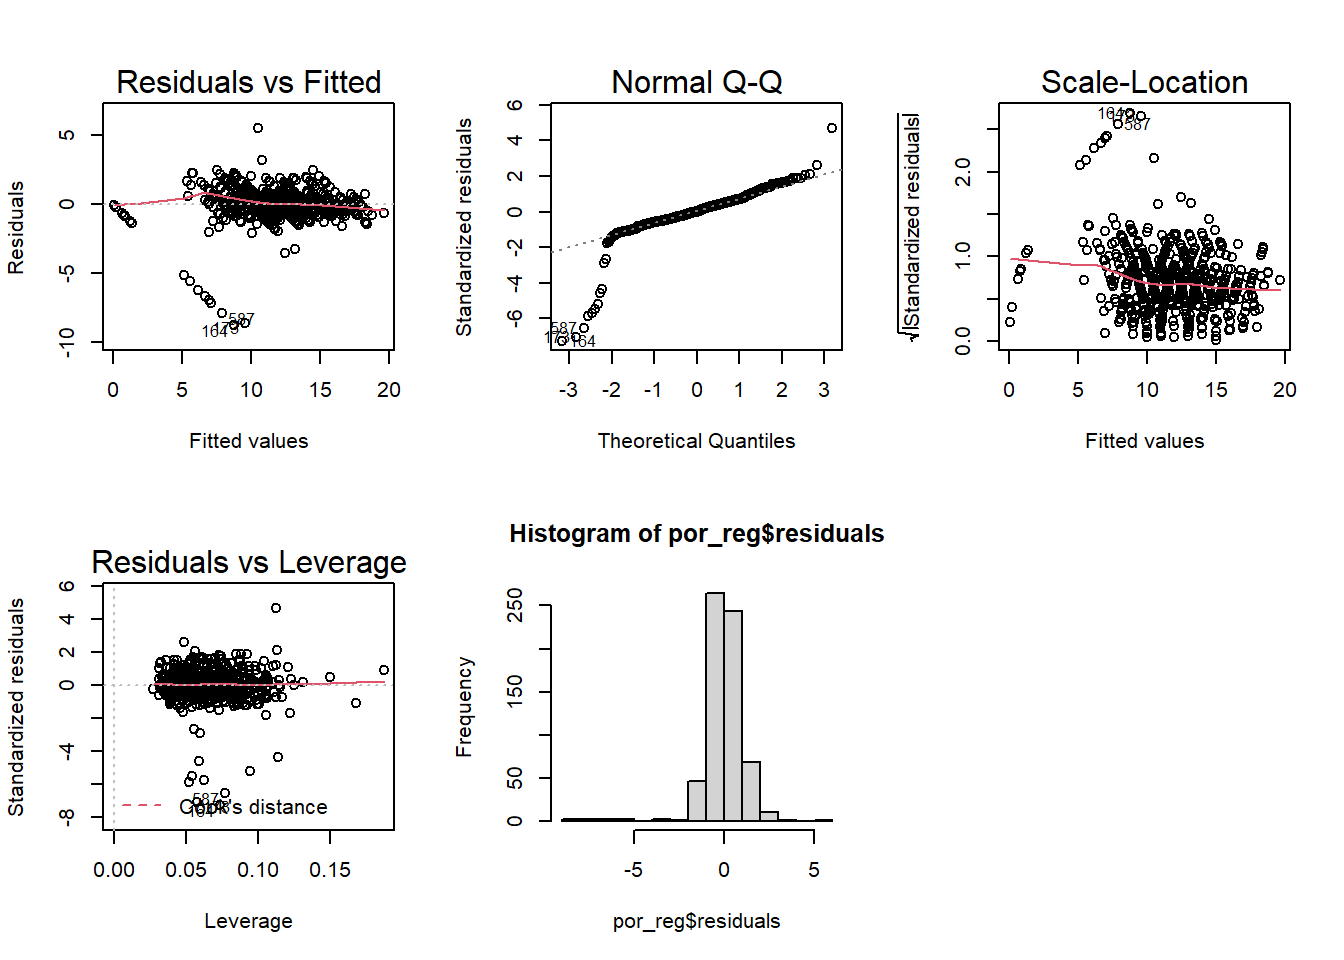
\includegraphics{report_files/figure-latex/unnamed-chunk-9-1.pdf}

We see that the residuals are not randomly distributed per the residual
plot and the QQ-plot yields residuals clearly left-skewed from
normality. Shapiro-Wilk test run on the residuals gives us the utmost
confidence that they do not have normal distribution. Future analysis
may seek to analyze the possible high-leverage points and potential
outliers as shown in the residuals vs.~leverage plot, but this is
outside the scope of this project and there are better-fitting methods
to consider.

\hypertarget{finding-linear-regression-mse}{%
\subsection{Finding Linear Regression
MSE}\label{finding-linear-regression-mse}}

Even though our initial model does not suit our needs, we can still
calculate the prediction MSE as a baseline to compare future models to,
anticipating that subsequent models will be more accurate.

\begin{Shaded}
\begin{Highlighting}[]
\FunctionTok{set.seed}\NormalTok{(}\DecValTok{1}\NormalTok{)}
\NormalTok{n }\OtherTok{\textless{}{-}} \FunctionTok{nrow}\NormalTok{(student\_por)}
\NormalTok{Z }\OtherTok{\textless{}{-}} \FunctionTok{sample}\NormalTok{(n, .}\DecValTok{7}\SpecialCharTok{*}\NormalTok{n)}

\NormalTok{reg.fit }\OtherTok{\textless{}{-}} \FunctionTok{lm}\NormalTok{(G3 }\SpecialCharTok{\textasciitilde{}}\NormalTok{ ., }\AttributeTok{data =}\NormalTok{ student\_por, }\AttributeTok{subset =}\NormalTok{ Z)}
\end{Highlighting}
\end{Shaded}

\begin{Shaded}
\begin{Highlighting}[]
\NormalTok{g3\_predicted }\OtherTok{\textless{}{-}} \FunctionTok{predict}\NormalTok{(reg.fit, student\_por)}
\end{Highlighting}
\end{Shaded}

\begin{Shaded}
\begin{Highlighting}[]
\FunctionTok{plot}\NormalTok{(student\_por}\SpecialCharTok{$}\NormalTok{G3[}\SpecialCharTok{{-}}\NormalTok{Z], g3\_predicted[}\SpecialCharTok{{-}}\NormalTok{Z], }\AttributeTok{xlab =} \StringTok{"Actual Grades"}\NormalTok{, }\AttributeTok{ylab =} \StringTok{"Predicted Grades"}\NormalTok{, }\AttributeTok{main =} \StringTok{"Prediction Accuracy of Full Linear Model"}\NormalTok{)}
\FunctionTok{abline}\NormalTok{(}\DecValTok{0}\NormalTok{,}\DecValTok{1}\NormalTok{)}
\end{Highlighting}
\end{Shaded}

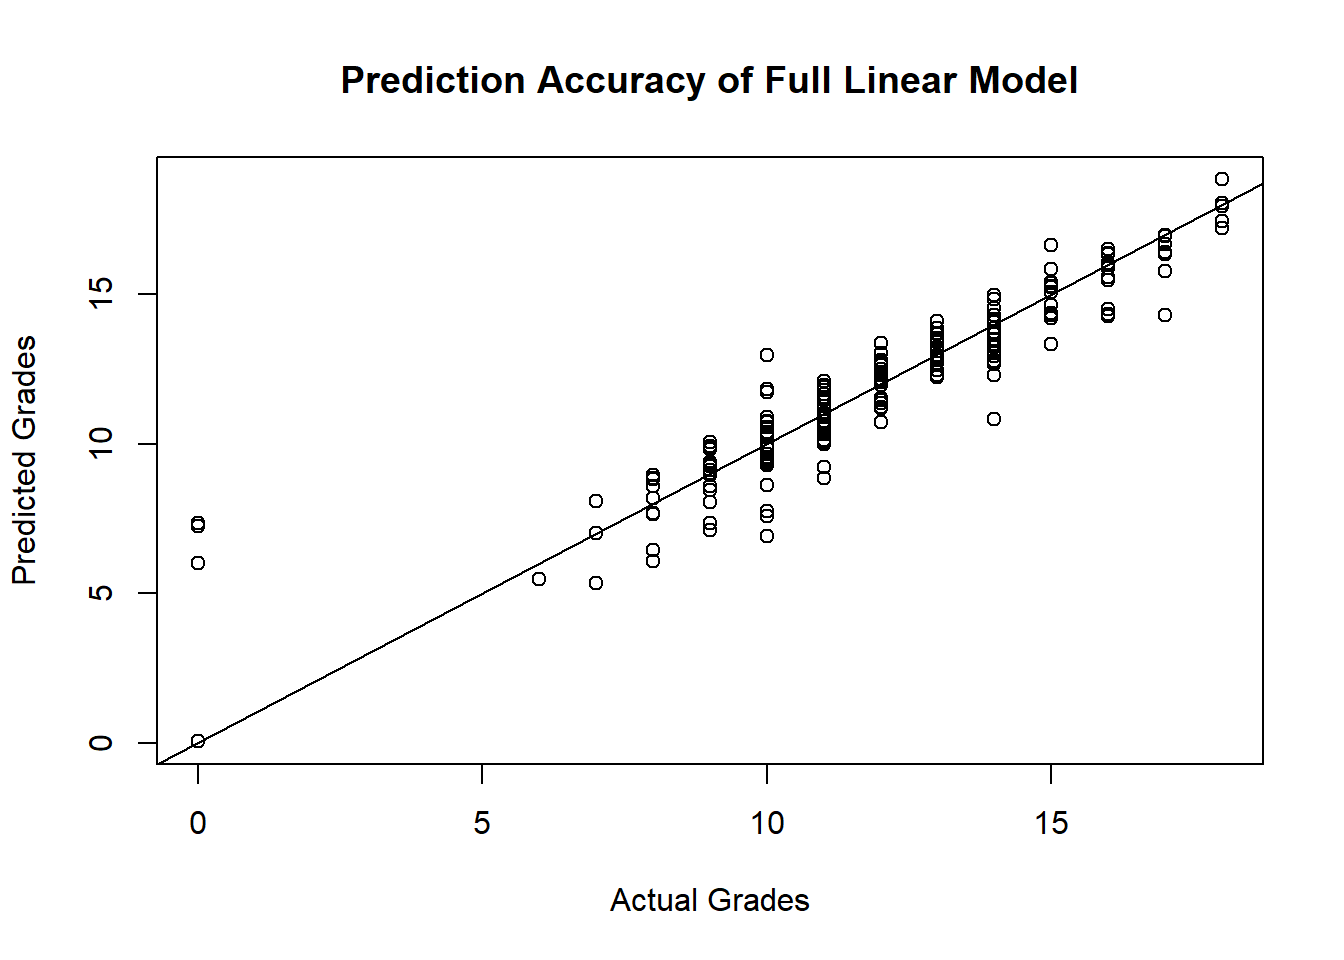
\includegraphics{report_files/figure-latex/unnamed-chunk-12-1.pdf}

We can see on the left side of the graph, when the actual G3 (final
grade) is 0, the model tends to overestimate.

\begin{Shaded}
\begin{Highlighting}[]
\NormalTok{mse\_lm }\OtherTok{\textless{}{-}} \FunctionTok{mean}\NormalTok{((student\_por}\SpecialCharTok{$}\NormalTok{G3 }\SpecialCharTok{{-}}\NormalTok{ g3\_predicted)[}\SpecialCharTok{{-}}\NormalTok{Z]}\SpecialCharTok{\^{}}\DecValTok{2}\NormalTok{)}
\NormalTok{mse\_lm}
\end{Highlighting}
\end{Shaded}

\begin{verbatim}
## [1] 1.549808
\end{verbatim}

Despite its flaws, the linear model has a rather low MSE (1.550) for
scores strictly on a 0-20 scale. When looking for a better model, we
will use methods in an attempt to reduce the number of variables or the
number of dimensions in the dataset. Therefore we will be using best
subset, forward and backwards step, LASSO, Ridge, PCR, and PLS. First,
we will start with Best Subset.

\hypertarget{best-subset}{%
\subsection{Best Subset}\label{best-subset}}

When initially running our best subset, we decided to cap the number of
variables at 15. This was done in order to ensure the model has enough
variables to predict G3 accurately without including unnecessary ones
that would complicate the model.

\begin{Shaded}
\begin{Highlighting}[]
\CommentTok{\# Takes a while to run}

\NormalTok{subsets }\OtherTok{\textless{}{-}} \FunctionTok{regsubsets}\NormalTok{(G3 }\SpecialCharTok{\textasciitilde{}}\NormalTok{ ., }\AttributeTok{data =}\NormalTok{ student\_por, }\AttributeTok{nvmax =} \DecValTok{15}\NormalTok{)}
\end{Highlighting}
\end{Shaded}

\begin{Shaded}
\begin{Highlighting}[]
\FunctionTok{summary}\NormalTok{(subsets)}\SpecialCharTok{$}\NormalTok{adjr2}
\end{Highlighting}
\end{Shaded}

\begin{verbatim}
##  [1] 0.8434889 0.8472902 0.8489562 0.8501271 0.8507762 0.8513288 0.8518147
##  [8] 0.8522527 0.8526228 0.8528667 0.8531441 0.8533129 0.8534618 0.8534808
## [15] 0.8535407
\end{verbatim}

\begin{Shaded}
\begin{Highlighting}[]
\FunctionTok{summary}\NormalTok{(subsets)}\SpecialCharTok{$}\NormalTok{cp}
\end{Highlighting}
\end{Shaded}

\begin{verbatim}
##  [1] 32.5841845 17.1053566 10.8932613  6.8369620  5.0413803  3.6686368
##  [7]  2.5898385  1.7227267  1.1515489  1.1240570  0.9573861  1.2563559
## [13]  1.6420508  2.5809380  3.3465888
\end{verbatim}

\begin{Shaded}
\begin{Highlighting}[]
\FunctionTok{summary}\NormalTok{(subsets)}\SpecialCharTok{$}\NormalTok{bic}
\end{Highlighting}
\end{Shaded}

\begin{verbatim}
##  [1] -1191.705 -1202.191 -1203.840 -1203.422 -1200.772 -1197.715 -1194.376
##  [8] -1190.835 -1187.002 -1182.618 -1178.385 -1173.676 -1168.881 -1163.512
## [15] -1158.327
\end{verbatim}

\hypertarget{set-validation-for-best-subset}{%
\subsection{Set validation for Best
Subset}\label{set-validation-for-best-subset}}

\hypertarget{best-subset-1}{%
\subsection{Best Subset}\label{best-subset-1}}

\begin{Shaded}
\begin{Highlighting}[]
\FunctionTok{which.max}\NormalTok{(}\FunctionTok{summary}\NormalTok{(subsets)}\SpecialCharTok{$}\NormalTok{adjr2)}
\end{Highlighting}
\end{Shaded}

\begin{verbatim}
## [1] 15
\end{verbatim}

\begin{Shaded}
\begin{Highlighting}[]
\FunctionTok{which.min}\NormalTok{(}\FunctionTok{abs}\NormalTok{(}\FunctionTok{summary}\NormalTok{(subsets)}\SpecialCharTok{$}\NormalTok{cp }\SpecialCharTok{{-}} \DecValTok{1}\SpecialCharTok{:}\DecValTok{15}\NormalTok{))}
\end{Highlighting}
\end{Shaded}

\begin{verbatim}
## [1] 5
\end{verbatim}

\begin{Shaded}
\begin{Highlighting}[]
\FunctionTok{which.min}\NormalTok{(}\FunctionTok{summary}\NormalTok{(subsets)}\SpecialCharTok{$}\NormalTok{bic)}
\end{Highlighting}
\end{Shaded}

\begin{verbatim}
## [1] 3
\end{verbatim}

When looking at the adjr2 value, we can tell that they are all
relatively the same, ranging from 0.843 to 0.854. Because adding in more
variables did not make a significant difference on this value, we are
not going to propose a candidate model based on the highest adjr2.
Instead, we will move forward with two candidate models, one with five
variables as suggested by the Mallow's Cp and one with three variables
as suggested by the BIC.

\hypertarget{model-based-on-mallows-cp}{%
\subsection{Model Based on Mallow's
Cp}\label{model-based-on-mallows-cp}}

Based on the output from Best Subset, we are going to run a model that
includes the variables: - sex - reason - failures - G1 - G2

\begin{Shaded}
\begin{Highlighting}[]
\NormalTok{reg.bestsubCP }\OtherTok{\textless{}{-}} \FunctionTok{lm}\NormalTok{(G3 }\SpecialCharTok{\textasciitilde{}}\NormalTok{ sex }\SpecialCharTok{+}\NormalTok{ reason }\SpecialCharTok{+}\NormalTok{ failures }\SpecialCharTok{+}\NormalTok{ G1 }\SpecialCharTok{+}\NormalTok{ G2, }\AttributeTok{data =}\NormalTok{ student\_por, }\AttributeTok{subset =}\NormalTok{ Z)}

\NormalTok{g3\_pred\_bestsubCP }\OtherTok{\textless{}{-}} \FunctionTok{predict}\NormalTok{(reg.bestsubCP, student\_por)}
\end{Highlighting}
\end{Shaded}

\begin{Shaded}
\begin{Highlighting}[]
\FunctionTok{plot}\NormalTok{(student\_por}\SpecialCharTok{$}\NormalTok{G3[}\SpecialCharTok{{-}}\NormalTok{Z], g3\_pred\_bestsubCP[}\SpecialCharTok{{-}}\NormalTok{Z], }\AttributeTok{xlab =} \StringTok{"Actual Grades"}\NormalTok{, }\AttributeTok{ylab =} \StringTok{"Predicted Grades"}\NormalTok{, }\AttributeTok{main =} \StringTok{"Predicted vs. Actual Grades of Reduced Model Based on Cp"}\NormalTok{)}
\FunctionTok{abline}\NormalTok{(}\DecValTok{0}\NormalTok{,}\DecValTok{1}\NormalTok{)}
\end{Highlighting}
\end{Shaded}

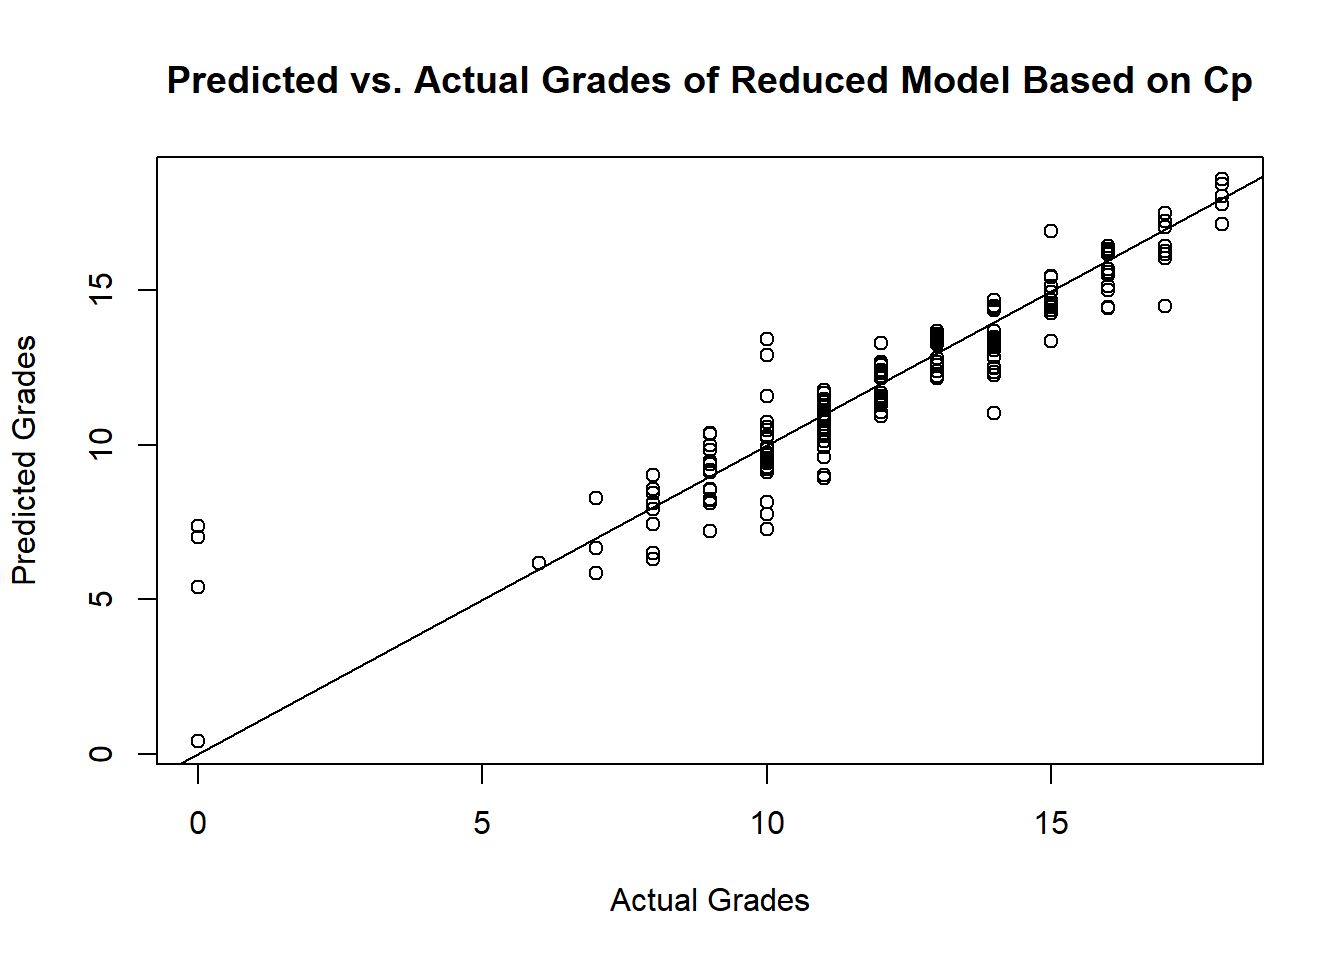
\includegraphics{report_files/figure-latex/unnamed-chunk-19-1.pdf}

Similar to the Predicted vs.~Actual Grade plot for the initial linear
regression, the Mallow's Cp model (with five variables) overestimates
the final grade (G3) when the actual grade is 0. These data points are
potential outliers, but removing them is outside of the scope of this
project. Otherwise, the model fits the rest of the data well.

\begin{Shaded}
\begin{Highlighting}[]
\NormalTok{mse\_cp }\OtherTok{\textless{}{-}} \FunctionTok{mean}\NormalTok{((student\_por}\SpecialCharTok{$}\NormalTok{G3 }\SpecialCharTok{{-}}\NormalTok{ g3\_pred\_bestsubCP)[}\SpecialCharTok{{-}}\NormalTok{Z] }\SpecialCharTok{\^{}} \DecValTok{2}\NormalTok{)}
\NormalTok{mse\_cp}
\end{Highlighting}
\end{Shaded}

\begin{verbatim}
## [1] 1.474193
\end{verbatim}

The MSE for the Best Subset Model based on Mallow's C is 1.474.

\hypertarget{model-based-on-bic}{%
\subsection{Model Based on BIC}\label{model-based-on-bic}}

Based on the output from Best Subset, we are going to run a model that
includes the variables: - reason - G1 - G2

\begin{Shaded}
\begin{Highlighting}[]
\NormalTok{reg.bestsubBIC }\OtherTok{\textless{}{-}} \FunctionTok{lm}\NormalTok{(G3 }\SpecialCharTok{\textasciitilde{}}\NormalTok{ reason }\SpecialCharTok{+}\NormalTok{ G1 }\SpecialCharTok{+}\NormalTok{ G2, }\AttributeTok{data =}\NormalTok{ student\_por, }\AttributeTok{subset =}\NormalTok{ Z)}

\NormalTok{g3\_pred\_bestsubBIC }\OtherTok{\textless{}{-}} \FunctionTok{predict}\NormalTok{(reg.bestsubBIC, student\_por)}
\end{Highlighting}
\end{Shaded}

\begin{Shaded}
\begin{Highlighting}[]
\FunctionTok{plot}\NormalTok{(student\_por}\SpecialCharTok{$}\NormalTok{G3[}\SpecialCharTok{{-}}\NormalTok{Z], g3\_pred\_bestsubBIC[}\SpecialCharTok{{-}}\NormalTok{Z], }\AttributeTok{xlab =} \StringTok{"Actual Grades"}\NormalTok{, }\AttributeTok{ylab =} \StringTok{"Predicted Grades"}\NormalTok{, }\AttributeTok{main =} \StringTok{"Predicted vs. Actual Grades of Reduced Model Based on BIC"}\NormalTok{)}
\FunctionTok{abline}\NormalTok{(}\DecValTok{0}\NormalTok{,}\DecValTok{1}\NormalTok{)}
\end{Highlighting}
\end{Shaded}

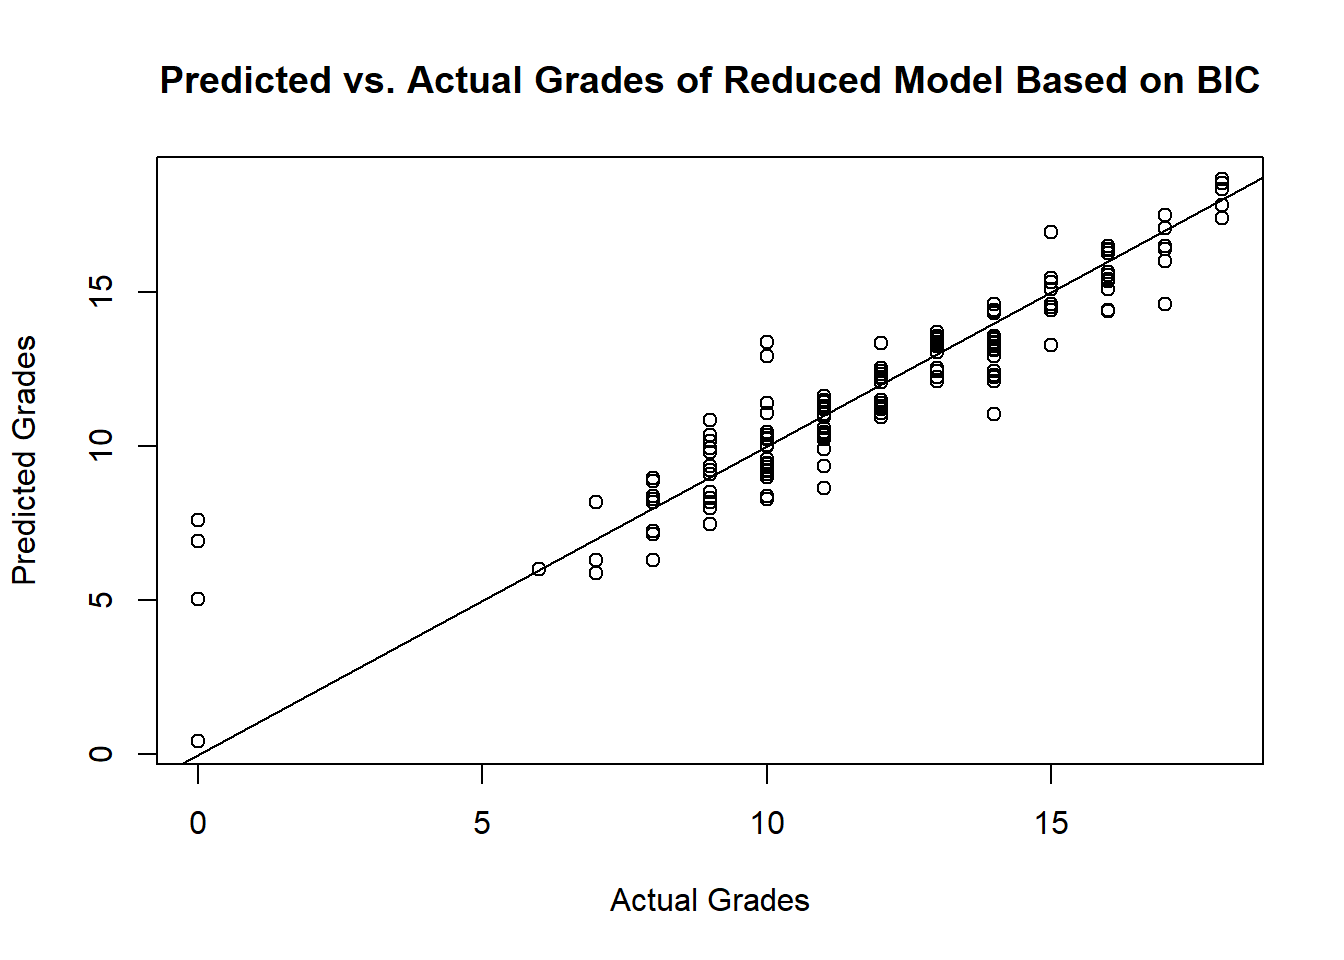
\includegraphics{report_files/figure-latex/unnamed-chunk-22-1.pdf}

Again, this plot is very similar to those for the previous models.

\begin{Shaded}
\begin{Highlighting}[]
\NormalTok{mse\_bic }\OtherTok{\textless{}{-}} \FunctionTok{mean}\NormalTok{((student\_por}\SpecialCharTok{$}\NormalTok{G3 }\SpecialCharTok{{-}}\NormalTok{ g3\_pred\_bestsubBIC)[}\SpecialCharTok{{-}}\NormalTok{Z] }\SpecialCharTok{\^{}} \DecValTok{2}\NormalTok{)}
\NormalTok{mse\_bic}
\end{Highlighting}
\end{Shaded}

\begin{verbatim}
## [1] 1.427079
\end{verbatim}

The MSE for the Best Subset Model based on BIC is 1.427.

\hypertarget{step-functions}{%
\subsection{Step Functions}\label{step-functions}}

Now we are going to be looking at forward and backward step functions.

\begin{Shaded}
\begin{Highlighting}[]
\FunctionTok{summary}\NormalTok{(forward)}
\end{Highlighting}
\end{Shaded}

\begin{verbatim}
## 
## Call:
## lm(formula = G3 ~ G2 + G1 + failures + reason + absences + sex + 
##     school + traveltime + health, data = student_por)
## 
## Residuals:
##     Min      1Q  Median      3Q     Max 
## -9.0833 -0.5178 -0.0053  0.6398  5.2097 
## 
## Coefficients:
##                  Estimate Std. Error t value Pr(>|t|)    
## (Intercept)       0.44063    0.34169   1.290 0.197678    
## G2                0.87996    0.03379  26.042  < 2e-16 ***
## G1                0.13706    0.03615   3.792 0.000164 ***
## failures         -0.24049    0.09074  -2.650 0.008244 ** 
## reasonhome       -0.09222    0.13010  -0.709 0.478659    
## reasonother      -0.44994    0.16627  -2.706 0.006990 ** 
## reasonreputation -0.16537    0.13290  -1.244 0.213816    
## absences          0.01623    0.01100   1.476 0.140522    
## sexM             -0.20022    0.10191  -1.965 0.049894 *  
## schoolMS         -0.22981    0.11621  -1.977 0.048419 *  
## traveltime        0.11228    0.06839   1.642 0.101138    
## health           -0.05394    0.03469  -1.555 0.120451    
## ---
## Signif. codes:  0 '***' 0.001 '**' 0.01 '*' 0.05 '.' 0.1 ' ' 1
## 
## Residual standard error: 1.242 on 637 degrees of freedom
## Multiple R-squared:  0.8547, Adjusted R-squared:  0.8522 
## F-statistic: 340.7 on 11 and 637 DF,  p-value: < 2.2e-16
\end{verbatim}

\begin{Shaded}
\begin{Highlighting}[]
\FunctionTok{summary}\NormalTok{(backward)}
\end{Highlighting}
\end{Shaded}

\begin{verbatim}
## 
## Call:
## lm(formula = G3 ~ school + sex + reason + traveltime + failures + 
##     health + absences + G1 + G2, data = student_por)
## 
## Residuals:
##     Min      1Q  Median      3Q     Max 
## -9.0833 -0.5178 -0.0053  0.6398  5.2097 
## 
## Coefficients:
##                  Estimate Std. Error t value Pr(>|t|)    
## (Intercept)       0.44063    0.34169   1.290 0.197678    
## schoolMS         -0.22981    0.11621  -1.977 0.048419 *  
## sexM             -0.20022    0.10191  -1.965 0.049894 *  
## reasonhome       -0.09222    0.13010  -0.709 0.478659    
## reasonother      -0.44994    0.16627  -2.706 0.006990 ** 
## reasonreputation -0.16537    0.13290  -1.244 0.213816    
## traveltime        0.11228    0.06839   1.642 0.101138    
## failures         -0.24049    0.09074  -2.650 0.008244 ** 
## health           -0.05394    0.03469  -1.555 0.120451    
## absences          0.01623    0.01100   1.476 0.140522    
## G1                0.13706    0.03615   3.792 0.000164 ***
## G2                0.87996    0.03379  26.042  < 2e-16 ***
## ---
## Signif. codes:  0 '***' 0.001 '**' 0.01 '*' 0.05 '.' 0.1 ' ' 1
## 
## Residual standard error: 1.242 on 637 degrees of freedom
## Multiple R-squared:  0.8547, Adjusted R-squared:  0.8522 
## F-statistic: 340.7 on 11 and 637 DF,  p-value: < 2.2e-16
\end{verbatim}

Forward and backward step functions yield the exact same model;
proceeding with forward step-generated model.

\hypertarget{set-validation}{%
\subsection{Set validation}\label{set-validation}}

Based on the output from Forward Step, we are going to run a model that
includes the variables: - failures - reason - absences - sex - school -
traveltime - health - G1 - G2

\begin{Shaded}
\begin{Highlighting}[]
\NormalTok{reg.forward }\OtherTok{\textless{}{-}} \FunctionTok{lm}\NormalTok{(G3 }\SpecialCharTok{\textasciitilde{}}\NormalTok{ G2 }\SpecialCharTok{+}\NormalTok{ G1 }\SpecialCharTok{+}\NormalTok{ failures }\SpecialCharTok{+}\NormalTok{ reason }\SpecialCharTok{+}\NormalTok{ absences }\SpecialCharTok{+}\NormalTok{ sex }\SpecialCharTok{+}\NormalTok{ school }\SpecialCharTok{+}\NormalTok{ traveltime }\SpecialCharTok{+}\NormalTok{ health, }\AttributeTok{data =}\NormalTok{ student\_por, }\AttributeTok{subset =}\NormalTok{ Z)}

\NormalTok{g3\_pred\_forward }\OtherTok{\textless{}{-}} \FunctionTok{predict}\NormalTok{(reg.forward, student\_por)}
\end{Highlighting}
\end{Shaded}

\begin{Shaded}
\begin{Highlighting}[]
\FunctionTok{plot}\NormalTok{(student\_por}\SpecialCharTok{$}\NormalTok{G3[}\SpecialCharTok{{-}}\NormalTok{Z], g3\_pred\_forward[}\SpecialCharTok{{-}}\NormalTok{Z], }\AttributeTok{xlab =} \StringTok{"Actual Grade"}\NormalTok{, }\AttributeTok{ylab =} \StringTok{"Predicted Grade"}\NormalTok{, }\AttributeTok{main =} \StringTok{"Actual vs. Predicted: Forward Step Model"}\NormalTok{)}
\FunctionTok{abline}\NormalTok{(}\DecValTok{0}\NormalTok{, }\DecValTok{1}\NormalTok{)}
\end{Highlighting}
\end{Shaded}

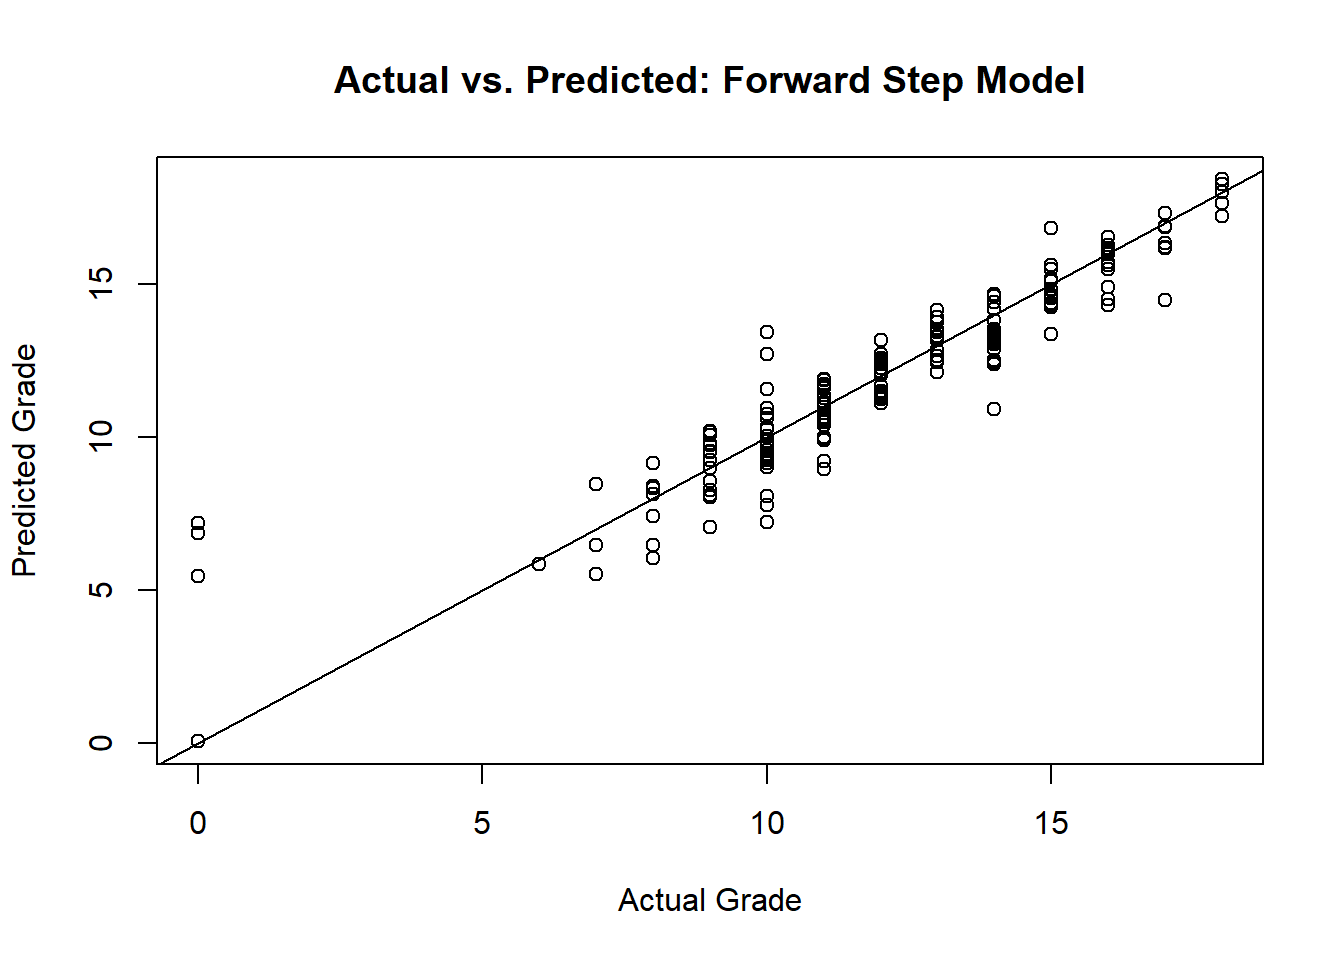
\includegraphics{report_files/figure-latex/unnamed-chunk-27-1.pdf}

\begin{Shaded}
\begin{Highlighting}[]
\NormalTok{mse\_valSet }\OtherTok{\textless{}{-}} \FunctionTok{mean}\NormalTok{((student\_por}\SpecialCharTok{$}\NormalTok{G3 }\SpecialCharTok{{-}}\NormalTok{ g3\_pred\_forward)[}\SpecialCharTok{{-}}\NormalTok{Z] }\SpecialCharTok{\^{}} \DecValTok{2}\NormalTok{)}
\NormalTok{mse\_valSet}
\end{Highlighting}
\end{Shaded}

\begin{verbatim}
## [1] 1.458564
\end{verbatim}

The MSE for the Forward STep Model is 1.459.

\hypertarget{ridge-regression-lasso-preparation}{%
\subsection{Ridge Regression \& LASSO
Preparation}\label{ridge-regression-lasso-preparation}}

\begin{Shaded}
\begin{Highlighting}[]
\NormalTok{G3\_test }\OtherTok{\textless{}{-}}\NormalTok{ student\_por}\SpecialCharTok{$}\NormalTok{G3[}\SpecialCharTok{{-}}\NormalTok{Z]}

\CommentTok{\# Creating model matrix for rr and lasso calculations}
\NormalTok{x\_col }\OtherTok{\textless{}{-}} \FunctionTok{model.matrix}\NormalTok{(G3 }\SpecialCharTok{\textasciitilde{}}\NormalTok{ ., student\_por)[, }\SpecialCharTok{{-}}\DecValTok{1}\NormalTok{]}
\end{Highlighting}
\end{Shaded}

\hypertarget{ridge-regression}{%
\subsection{Ridge Regression}\label{ridge-regression}}

Now we are going to look at Ridge Regression.

\begin{Shaded}
\begin{Highlighting}[]
\FunctionTok{set.seed}\NormalTok{(}\DecValTok{1}\NormalTok{)}
\NormalTok{cv.out1 }\OtherTok{\textless{}{-}} \FunctionTok{cv.glmnet}\NormalTok{(x\_col, student\_por}\SpecialCharTok{$}\NormalTok{G3, }\AttributeTok{alpha =} \DecValTok{0}\NormalTok{) }\CommentTok{\# alpha = 0 {-}{-}{-}\textgreater{} Ridge regression}
\FunctionTok{predict}\NormalTok{(cv.out1, }\AttributeTok{s =}\NormalTok{ cv.out1}\SpecialCharTok{$}\NormalTok{lambda.min, }\AttributeTok{type =} \StringTok{"coefficients"}\NormalTok{)}
\end{Highlighting}
\end{Shaded}

\begin{verbatim}
## 42 x 1 sparse Matrix of class "dgCMatrix"
##                             1
## (Intercept)       0.647281475
## schoolMS         -0.203906036
## sexM             -0.140157325
## age               0.052338494
## addressU          0.134471281
## famsizeLE3        0.031162924
## PstatusT         -0.065759455
## Medu             -0.052585350
## Fedu              0.042315840
## Mjobhealth        0.214144623
## Mjobother        -0.125812519
## Mjobservices      0.107348800
## Mjobteacher       0.126800272
## Fjobhealth       -0.238572263
## Fjobother        -0.156282858
## Fjobservices     -0.300920468
## Fjobteacher      -0.249881588
## reasonhome       -0.066205753
## reasonother      -0.362017744
## reasonreputation -0.112276025
## guardianmother   -0.032801219
## guardianother     0.212481561
## traveltime        0.111686852
## studytime         0.060781281
## failures         -0.316944745
## schoolsupyes     -0.201688220
## famsupyes         0.087520158
## paidyes          -0.153298259
## activitiesyes     0.018965743
## nurseryyes       -0.084879671
## higheryes         0.280580244
## internetyes       0.099020055
## romanticyes      -0.087129209
## famrel            0.008539498
## freetime         -0.053552694
## goout            -0.025522281
## Dalc             -0.056693604
## Walc             -0.025883700
## health           -0.065912944
## absences          0.011871609
## G1                0.258399918
## G2                0.683417827
\end{verbatim}

\begin{Shaded}
\begin{Highlighting}[]
\NormalTok{rr.mod }\OtherTok{\textless{}{-}} \FunctionTok{glmnet}\NormalTok{(x\_col[Z, ], student\_por}\SpecialCharTok{$}\NormalTok{G3[Z], }\AttributeTok{alpha =} \DecValTok{0}\NormalTok{, }\AttributeTok{lambda =}\NormalTok{ cv.out1}\SpecialCharTok{$}\NormalTok{lambda.min)}
\NormalTok{rr.pred }\OtherTok{\textless{}{-}} \FunctionTok{predict}\NormalTok{(rr.mod, }\AttributeTok{s =}\NormalTok{ cv.out1}\SpecialCharTok{$}\NormalTok{lambda.min, }\AttributeTok{newx =}\NormalTok{ x\_col[}\SpecialCharTok{{-}}\NormalTok{Z, ])}

\NormalTok{mse\_rr }\OtherTok{\textless{}{-}} \FunctionTok{mean}\NormalTok{((rr.pred }\SpecialCharTok{{-}}\NormalTok{ student\_por}\SpecialCharTok{$}\NormalTok{G3[}\SpecialCharTok{{-}}\NormalTok{Z])}\SpecialCharTok{\^{}}\DecValTok{2}\NormalTok{)}
\NormalTok{mse\_rr}
\end{Highlighting}
\end{Shaded}

\begin{verbatim}
## [1] 1.596999
\end{verbatim}

The MSE for Ridge Regression is 1.597.

\(\lambda = .30\)

\hypertarget{lasso}{%
\subsection{LASSO}\label{lasso}}

Next we are going to look at LASSO.

\begin{Shaded}
\begin{Highlighting}[]
\FunctionTok{set.seed}\NormalTok{(}\DecValTok{1}\NormalTok{)}
\NormalTok{cv.out2 }\OtherTok{\textless{}{-}} \FunctionTok{cv.glmnet}\NormalTok{(x\_col, student\_por}\SpecialCharTok{$}\NormalTok{G3, }\AttributeTok{alpha =} \DecValTok{1}\NormalTok{)}
\FunctionTok{predict}\NormalTok{(cv.out2, }\AttributeTok{s =}\NormalTok{ cv.out2}\SpecialCharTok{$}\NormalTok{lambda.min, }\AttributeTok{type =} \StringTok{"coefficients"}\NormalTok{)}
\end{Highlighting}
\end{Shaded}

\begin{verbatim}
## 42 x 1 sparse Matrix of class "dgCMatrix"
##                            1
## (Intercept)       0.46985582
## schoolMS         -0.03190401
## sexM             -0.01841156
## age               .         
## addressU          .         
## famsizeLE3        .         
## PstatusT          .         
## Medu              .         
## Fedu              .         
## Mjobhealth        .         
## Mjobother         .         
## Mjobservices      .         
## Mjobteacher       .         
## Fjobhealth        .         
## Fjobother         .         
## Fjobservices      .         
## Fjobteacher       .         
## reasonhome        .         
## reasonother      -0.14557639
## reasonreputation  .         
## guardianmother    .         
## guardianother     .         
## traveltime        .         
## studytime         .         
## failures         -0.09120067
## schoolsupyes      .         
## famsupyes         .         
## paidyes           .         
## activitiesyes     .         
## nurseryyes        .         
## higheryes         .         
## internetyes       .         
## romanticyes       .         
## famrel            .         
## freetime          .         
## goout             .         
## Dalc              .         
## Walc              .         
## health            .         
## absences          .         
## G1                0.12252007
## G2                0.87247067
\end{verbatim}

\(\lambda = .10\)

\begin{Shaded}
\begin{Highlighting}[]
\NormalTok{lasso.mod }\OtherTok{\textless{}{-}} \FunctionTok{glmnet}\NormalTok{(x\_col[Z, ], student\_por}\SpecialCharTok{$}\NormalTok{G3[Z], }\AttributeTok{alpha =} \DecValTok{1}\NormalTok{, }\AttributeTok{lambda =}\NormalTok{ cv.out2}\SpecialCharTok{$}\NormalTok{lambda.min)}
\NormalTok{lasso.pred }\OtherTok{\textless{}{-}} \FunctionTok{predict}\NormalTok{(lasso.mod, }\AttributeTok{s =}\NormalTok{ cv.out2}\SpecialCharTok{$}\NormalTok{lambda.min, }\AttributeTok{newx =}\NormalTok{ x\_col[}\SpecialCharTok{{-}}\NormalTok{Z, ])}

\NormalTok{mse\_lasso }\OtherTok{\textless{}{-}} \FunctionTok{mean}\NormalTok{((lasso.pred }\SpecialCharTok{{-}}\NormalTok{ student\_por}\SpecialCharTok{$}\NormalTok{G3[}\SpecialCharTok{{-}}\NormalTok{Z])}\SpecialCharTok{\^{}}\DecValTok{2}\NormalTok{)}
\NormalTok{mse\_lasso}
\end{Highlighting}
\end{Shaded}

\begin{verbatim}
## [1] 1.527916
\end{verbatim}

The MSE for Lasso is 1.528.

\hypertarget{principal-component-regression}{%
\subsection{Principal Component
Regression}\label{principal-component-regression}}

Now we are going to look at principal component regression.

\begin{Shaded}
\begin{Highlighting}[]
\NormalTok{pcr.fit }\OtherTok{\textless{}{-}} \FunctionTok{pcr}\NormalTok{(G3 }\SpecialCharTok{\textasciitilde{}}\NormalTok{ ., }\AttributeTok{data =}\NormalTok{ student\_por, }\AttributeTok{scale =} \ConstantTok{TRUE}\NormalTok{, }\AttributeTok{validation =} \StringTok{"CV"}\NormalTok{)}
\FunctionTok{summary}\NormalTok{(pcr.fit)}
\end{Highlighting}
\end{Shaded}

\begin{verbatim}
## Data:    X dimension: 649 41 
##  Y dimension: 649 1
## Fit method: svdpc
## Number of components considered: 41
## 
## VALIDATION: RMSEP
## Cross-validated using 10 random segments.
##        (Intercept)  1 comps  2 comps  3 comps  4 comps  5 comps  6 comps
## CV           3.233    2.426    2.289    2.249    2.236    2.065    2.021
## adjCV        3.233    2.425    2.287    2.248    2.233    2.018    2.029
##        7 comps  8 comps  9 comps  10 comps  11 comps  12 comps  13 comps
## CV       1.877    1.866    1.863     1.869     1.851     1.827     1.795
## adjCV    1.857    1.853    1.858     1.865     1.859     1.825     1.797
##        14 comps  15 comps  16 comps  17 comps  18 comps  19 comps  20 comps
## CV        1.739     1.728     1.720     1.727     1.708     1.661     1.652
## adjCV     1.735     1.719     1.711     1.725     1.706     1.644     1.649
##        21 comps  22 comps  23 comps  24 comps  25 comps  26 comps  27 comps
## CV        1.639     1.632     1.600     1.578     1.542     1.534     1.522
## adjCV     1.632     1.632     1.603     1.575     1.531     1.529     1.518
##        28 comps  29 comps  30 comps  31 comps  32 comps  33 comps  34 comps
## CV        1.528     1.494     1.463     1.454     1.452     1.430     1.428
## adjCV     1.528     1.496     1.457     1.451     1.449     1.423     1.424
##        35 comps  36 comps  37 comps  38 comps  39 comps  40 comps  41 comps
## CV        1.405     1.407     1.404     1.407     1.410     1.292     1.293
## adjCV     1.400     1.403     1.400     1.402     1.406     1.287     1.289
## 
## TRAINING: % variance explained
##     1 comps  2 comps  3 comps  4 comps  5 comps  6 comps  7 comps  8 comps
## X     9.881    16.40    21.46    25.82    29.83    33.72    37.44    40.94
## G3   44.250    50.22    52.25    52.96    61.41    61.59    67.57    67.77
##     9 comps  10 comps  11 comps  12 comps  13 comps  14 comps  15 comps
## X     44.35     47.48     50.46     53.39     56.21     58.93     61.46
## G3    67.77     67.79     68.50     70.12     70.91     73.25     73.85
##     16 comps  17 comps  18 comps  19 comps  20 comps  21 comps  22 comps
## X      63.92     66.31     68.61     70.84     73.05     75.09     77.07
## G3     74.12     74.14     74.72     76.16     76.18     76.83     77.03
##     23 comps  24 comps  25 comps  26 comps  27 comps  28 comps  29 comps
## X      78.97     80.82     82.59     84.25     85.89     87.47     89.00
## G3     77.62     78.59     79.77     79.99     80.21     80.40     81.05
##     30 comps  31 comps  32 comps  33 comps  34 comps  35 comps  36 comps
## X      90.49     91.87     93.17     94.35     95.48     96.53     97.52
## G3     81.83     81.87     81.91     82.52     82.64     83.12     83.13
##     37 comps  38 comps  39 comps  40 comps  41 comps
## X      98.38     99.05     99.46     99.76       100
## G3     83.18     83.19     83.21     85.97        86
\end{verbatim}

\begin{Shaded}
\begin{Highlighting}[]
\NormalTok{R2.pcr }\OtherTok{=} \FunctionTok{as.numeric}\NormalTok{(}\FunctionTok{R2}\NormalTok{(pcr.fit, }\AttributeTok{estimate=}\StringTok{"train"}\NormalTok{)}\SpecialCharTok{$}\NormalTok{val)}
\NormalTok{mse.pcr }\OtherTok{=} \FunctionTok{as.numeric}\NormalTok{(}\FunctionTok{MSEP}\NormalTok{(pcr.fit, }\AttributeTok{estimate=}\StringTok{"train"}\NormalTok{)}\SpecialCharTok{$}\NormalTok{val)}

\NormalTok{R2.pcr}
\end{Highlighting}
\end{Shaded}

\begin{verbatim}
##  [1] 0.0000000 0.4425048 0.5021809 0.5224846 0.5296433 0.6140847 0.6159433
##  [8] 0.6757365 0.6777191 0.6777401 0.6779114 0.6850131 0.7011920 0.7091014
## [15] 0.7324872 0.7384674 0.7411768 0.7413506 0.7472237 0.7615905 0.7617913
## [22] 0.7682921 0.7702811 0.7761945 0.7858873 0.7976724 0.7999222 0.8020673
## [29] 0.8040197 0.8104576 0.8183151 0.8186857 0.8191378 0.8251620 0.8264211
## [36] 0.8312160 0.8313354 0.8318378 0.8319371 0.8321284 0.8597183 0.8600091
\end{verbatim}

\begin{Shaded}
\begin{Highlighting}[]
\NormalTok{mse.pcr}
\end{Highlighting}
\end{Shaded}

\begin{verbatim}
##  [1] 10.421058  5.809689  5.187802  4.976215  4.901614  4.021646  4.002277
##  [8]  3.379169  3.358508  3.358289  3.356504  3.282497  3.113895  3.031471
## [15]  2.787767  2.725447  2.697211  2.695401  2.634196  2.484479  2.482387
## [22]  2.414641  2.393914  2.332290  2.231281  2.108468  2.085022  2.062668
## [29]  2.042322  1.975232  1.893349  1.889487  1.884775  1.821997  1.808875
## [36]  1.758908  1.757664  1.752428  1.751393  1.749400  1.461884  1.458853
\end{verbatim}

PCR attains the lowest prediction MSE = 1.458 when all 41 principal
components are included. This result, which would be overly cumbersome
to analyze within this project's scope, does not lend itself well to
further analysis compared to more dimension-reduced models. If we were
to compromise the number of principal components, we would still need to
include 20+ to create a model with an MSE that is comparable to our
previous models. Therefore, we will not be suggesting a candidate model
based on principal component regression.

\hypertarget{partial-least-squares-regression}{%
\subsection{Partial Least Squares
Regression}\label{partial-least-squares-regression}}

\begin{Shaded}
\begin{Highlighting}[]
\NormalTok{pls.fit }\OtherTok{\textless{}{-}} \FunctionTok{plsr}\NormalTok{(G3 }\SpecialCharTok{\textasciitilde{}}\NormalTok{ ., }\AttributeTok{data =}\NormalTok{ student\_por, }\AttributeTok{scale =} \ConstantTok{TRUE}\NormalTok{, }\AttributeTok{validation =} \StringTok{"CV"}\NormalTok{)}
\FunctionTok{summary}\NormalTok{(pls.fit)}
\end{Highlighting}
\end{Shaded}

\begin{verbatim}
## Data:    X dimension: 649 41 
##  Y dimension: 649 1
## Fit method: kernelpls
## Number of components considered: 41
## 
## VALIDATION: RMSEP
## Cross-validated using 10 random segments.
##        (Intercept)  1 comps  2 comps  3 comps  4 comps  5 comps  6 comps
## CV           3.233    1.869    1.482    1.410    1.378    1.362    1.345
## adjCV        3.233    1.867    1.476    1.404    1.372    1.355    1.338
##        7 comps  8 comps  9 comps  10 comps  11 comps  12 comps  13 comps
## CV       1.329    1.325    1.323     1.323     1.322     1.322     1.322
## adjCV    1.322    1.319    1.317     1.317     1.316     1.316     1.316
##        14 comps  15 comps  16 comps  17 comps  18 comps  19 comps  20 comps
## CV        1.322     1.322     1.322     1.322     1.322     1.322     1.322
## adjCV     1.316     1.316     1.316     1.316     1.316     1.316     1.316
##        21 comps  22 comps  23 comps  24 comps  25 comps  26 comps  27 comps
## CV        1.322     1.322     1.322     1.322     1.322     1.322     1.322
## adjCV     1.316     1.316     1.316     1.316     1.316     1.316     1.316
##        28 comps  29 comps  30 comps  31 comps  32 comps  33 comps  34 comps
## CV        1.322     1.322     1.322     1.322     1.322     1.322     1.322
## adjCV     1.316     1.316     1.316     1.316     1.316     1.316     1.316
##        35 comps  36 comps  37 comps  38 comps  39 comps  40 comps  41 comps
## CV        1.322     1.322     1.322     1.322     1.322     1.322     1.322
## adjCV     1.316     1.316     1.316     1.316     1.316     1.316     1.316
## 
## TRAINING: % variance explained
##     1 comps  2 comps  3 comps  4 comps  5 comps  6 comps  7 comps  8 comps
## X     9.252    13.87    18.53    22.04    24.79    27.69    30.06    32.51
## G3   68.458    81.36    83.60    84.60    85.24    85.70    85.94    85.99
##     9 comps  10 comps  11 comps  12 comps  13 comps  14 comps  15 comps
## X     35.36     37.87     40.78     42.82     44.51     46.38     48.35
## G3    86.00     86.00     86.00     86.00     86.00     86.00     86.00
##     16 comps  17 comps  18 comps  19 comps  20 comps  21 comps  22 comps
## X      50.64     52.41     54.81     56.98     58.71     60.58     62.49
## G3     86.00     86.00     86.00     86.00     86.00     86.00     86.00
##     23 comps  24 comps  25 comps  26 comps  27 comps  28 comps  29 comps
## X      64.48     66.68     69.15     71.33     73.58     75.51     77.53
## G3     86.00     86.00     86.00     86.00     86.00     86.00     86.00
##     30 comps  31 comps  32 comps  33 comps  34 comps  35 comps  36 comps
## X      79.56     81.64     83.31     85.29        87     88.77     90.56
## G3     86.00     86.00     86.00     86.00        86     86.00     86.00
##     37 comps  38 comps  39 comps  40 comps  41 comps
## X      92.63     94.45     96.32     98.35       100
## G3     86.00     86.00     86.00     86.00        86
\end{verbatim}

\begin{Shaded}
\begin{Highlighting}[]
\NormalTok{R2.pls }\OtherTok{=} \FunctionTok{as.numeric}\NormalTok{(}\FunctionTok{R2}\NormalTok{(pls.fit, }\AttributeTok{estimate=}\StringTok{"train"}\NormalTok{)}\SpecialCharTok{$}\NormalTok{val)}
\NormalTok{mse.pls }\OtherTok{=} \FunctionTok{as.numeric}\NormalTok{(}\FunctionTok{MSEP}\NormalTok{(pls.fit, }\AttributeTok{estimate=}\StringTok{"train"}\NormalTok{)}\SpecialCharTok{$}\NormalTok{val)}

\NormalTok{R2.pls}
\end{Highlighting}
\end{Shaded}

\begin{verbatim}
##  [1] 0.0000000 0.6845804 0.8136119 0.8360447 0.8459948 0.8524414 0.8570038
##  [8] 0.8594111 0.8599011 0.8599891 0.8600032 0.8600060 0.8600076 0.8600085
## [15] 0.8600089 0.8600090 0.8600091 0.8600091 0.8600091 0.8600091 0.8600091
## [22] 0.8600091 0.8600091 0.8600091 0.8600091 0.8600091 0.8600091 0.8600091
## [29] 0.8600091 0.8600091 0.8600091 0.8600091 0.8600091 0.8600091 0.8600091
## [36] 0.8600091 0.8600091 0.8600091 0.8600091 0.8600091 0.8600091 0.8600091
\end{verbatim}

\begin{Shaded}
\begin{Highlighting}[]
\NormalTok{mse.pls}
\end{Highlighting}
\end{Shaded}

\begin{verbatim}
##  [1] 10.421058  3.287006  1.942361  1.708588  1.604897  1.537717  1.490172
##  [8]  1.465085  1.459978  1.459062  1.458915  1.458886  1.458869  1.458860
## [15]  1.458856  1.458854  1.458854  1.458853  1.458853  1.458853  1.458853
## [22]  1.458853  1.458853  1.458853  1.458853  1.458853  1.458853  1.458853
## [29]  1.458853  1.458853  1.458853  1.458853  1.458853  1.458853  1.458853
## [36]  1.458853  1.458853  1.458853  1.458853  1.458853  1.458853  1.458853
\end{verbatim}

\begin{Shaded}
\begin{Highlighting}[]
\NormalTok{mse.pls }\OtherTok{\textless{}{-}}\NormalTok{ mse.pls[}\DecValTok{10}\NormalTok{]}
\end{Highlighting}
\end{Shaded}

PLS attains the lowest predict MSE = 1.458853 with 18 principal
components. If we were going to consider one of these models as a
candidate model, I would consider sacrificing a little prediction
accuracy for simplicity/dimension reduction. I would recommend using the
model with 10 principal components because the MSE is 1.459062 which is
only slightly higher than that with 18 with 8 fewer principal
components.

\hypertarget{comparing-mses}{%
\subsection{Comparing MSEs}\label{comparing-mses}}

Now that we have proposed all of our candidate models, we are going to
take a look at the MSE to determine our final model.

\begin{Shaded}
\begin{Highlighting}[]
\FunctionTok{tibble}\NormalTok{(}\StringTok{"method"} \OtherTok{=} \FunctionTok{c}\NormalTok{(}\StringTok{"BIC{-}Minimized"}\NormalTok{, }\StringTok{"Cp{-}Minimized"}\NormalTok{, }\StringTok{"LASSO"}\NormalTok{, }\StringTok{"Linear Regression"}\NormalTok{, }\StringTok{"Ridge Regression"}\NormalTok{, }\StringTok{"AIC{-}Minimized"}\NormalTok{, }\StringTok{"PLS"}\NormalTok{),}
       \StringTok{"MSE"} \OtherTok{=} \FunctionTok{c}\NormalTok{(mse\_bic, mse\_cp, mse\_lasso, mse\_lm, mse\_rr, mse\_valSet, mse.pls)) }\SpecialCharTok{\%\textgreater{}\%}
  \FunctionTok{arrange}\NormalTok{(MSE)}
\end{Highlighting}
\end{Shaded}

\begin{verbatim}
## # A tibble: 7 x 2
##   method              MSE
##   <chr>             <dbl>
## 1 BIC-Minimized      1.43
## 2 AIC-Minimized      1.46
## 3 PLS                1.46
## 4 Cp-Minimized       1.47
## 5 LASSO              1.53
## 6 Linear Regression  1.55
## 7 Ridge Regression   1.60
\end{verbatim}

Based on the MSE, we are going to examine the top three models and
determine which one has the best balance of number of predictors and
accuracy.

\begin{Shaded}
\begin{Highlighting}[]
\NormalTok{reg.bestsubBIC}
\end{Highlighting}
\end{Shaded}

\begin{verbatim}
## 
## Call:
## lm(formula = G3 ~ reason + G1 + G2, data = student_por, subset = Z)
## 
## Coefficients:
##      (Intercept)        reasonhome       reasonother  reasonreputation  
##         -0.01247          -0.08366          -0.33815          -0.10231  
##               G1                G2  
##          0.10995           0.92593
\end{verbatim}

\begin{Shaded}
\begin{Highlighting}[]
\NormalTok{reg.forward }\CommentTok{\# Picking this one}
\end{Highlighting}
\end{Shaded}

\begin{verbatim}
## 
## Call:
## lm(formula = G3 ~ G2 + G1 + failures + reason + absences + sex + 
##     school + traveltime + health, data = student_por, subset = Z)
## 
## Coefficients:
##      (Intercept)                G2                G1          failures  
##          0.50898           0.90144           0.09950          -0.37556  
##       reasonhome       reasonother  reasonreputation          absences  
##         -0.13167          -0.33802          -0.21118           0.01524  
##             sexM          schoolMS        traveltime            health  
##         -0.20738          -0.22059           0.16919          -0.04444
\end{verbatim}

Picking forward-selected candidate model because best balance of number
of predictors while sacrificing only a little accuracy.

\hypertarget{conclusion}{%
\section{Conclusion}\label{conclusion}}

After examining a variety of candidate models, we have decided to use
the model generated by forward step selection. We believe that this
model does not eliminate too many variables while maintaining a
relatively low MSE of 1.459. We have run the model again with the full
data set below.

\begin{Shaded}
\begin{Highlighting}[]
\NormalTok{reg.forward\_full }\OtherTok{\textless{}{-}} \FunctionTok{lm}\NormalTok{(G3 }\SpecialCharTok{\textasciitilde{}}\NormalTok{ G1 }\SpecialCharTok{+}\NormalTok{ G2 }\SpecialCharTok{+}\NormalTok{ failures }\SpecialCharTok{+}\NormalTok{ reason }\SpecialCharTok{+}\NormalTok{ absences }\SpecialCharTok{+}\NormalTok{ sex }\SpecialCharTok{+}\NormalTok{ school }\SpecialCharTok{+}\NormalTok{ traveltime }\SpecialCharTok{+}\NormalTok{ health, student\_por)}

\FunctionTok{summary}\NormalTok{(reg.forward\_full)}
\end{Highlighting}
\end{Shaded}

\begin{verbatim}
## 
## Call:
## lm(formula = G3 ~ G1 + G2 + failures + reason + absences + sex + 
##     school + traveltime + health, data = student_por)
## 
## Residuals:
##     Min      1Q  Median      3Q     Max 
## -9.0833 -0.5178 -0.0053  0.6398  5.2097 
## 
## Coefficients:
##                  Estimate Std. Error t value Pr(>|t|)    
## (Intercept)       0.44063    0.34169   1.290 0.197678    
## G1                0.13706    0.03615   3.792 0.000164 ***
## G2                0.87996    0.03379  26.042  < 2e-16 ***
## failures         -0.24049    0.09074  -2.650 0.008244 ** 
## reasonhome       -0.09222    0.13010  -0.709 0.478659    
## reasonother      -0.44994    0.16627  -2.706 0.006990 ** 
## reasonreputation -0.16537    0.13290  -1.244 0.213816    
## absences          0.01623    0.01100   1.476 0.140522    
## sexM             -0.20022    0.10191  -1.965 0.049894 *  
## schoolMS         -0.22981    0.11621  -1.977 0.048419 *  
## traveltime        0.11228    0.06839   1.642 0.101138    
## health           -0.05394    0.03469  -1.555 0.120451    
## ---
## Signif. codes:  0 '***' 0.001 '**' 0.01 '*' 0.05 '.' 0.1 ' ' 1
## 
## Residual standard error: 1.242 on 637 degrees of freedom
## Multiple R-squared:  0.8547, Adjusted R-squared:  0.8522 
## F-statistic: 340.7 on 11 and 637 DF,  p-value: < 2.2e-16
\end{verbatim}

Our final model is as follows:

\[ \widehat{G3} = 0.441 + 0.137 (G1) + 0.880 (G2) -0.240(failures) - 0.092(reasonhome) - 0.450(reasonother) - 0.165(reasonrep) + 0.016(absences) - 0.200(sexMale) - 0.230(schoolMS) + 0.112(traveltime) - 0.054(health)\]

Let's look at each of these variables and what they mean.

\begin{itemize}
\tightlist
\item
  G1 is the student's grade during the first term
\item
  G2 is the student's grade during the second term
\item
  Failures is the number of past class failures a student had
\item
  Reason is the reason a student attended a certain school
\item
  Absences is the number of absences a student had
\item
  Sex is the sex of the student
\item
  School is a the name of the school the student attended
\item
  Traveltime is the amount of time it took a student to get to school
\item
  Health is the current health status of the student
\end{itemize}

Based on our final model, these are the variables that are significant
when attempting to predict a student's final grade in Portuguese class
(G3).

\end{document}
